\chapter{Derivative of Vector}

\section{一元泰勒展开}

我们知道函数的一阶导数表示函数在一点的斜率,这意味着函数在这一点的斜率行为可以用一条切线逼近
\begin{equation}
    f(x)=f(x_0)+f'(x_0)(x-x_0)
\end{equation}

这可以看作是一个一元多项式,因此能够想到如果想更多描述函数在某点处的行为(比如描述函数斜率的变化率还需要知道二阶导数)可以用多项式去逼近,这就是泰勒开展
\begin{equation}
    f(x)=f(x_0)+f^{(1)}(x_0)(x-x_0)+\frac{f^{(2)}}{2!}(x-x_0)^2+\cdots+\frac{f^{(n)}}{n!}(x-x_0)^n+o((x-x_0)^{n+1})
\end{equation}

\section{二元泰勒展开}

定义点$(a_1,a_2)$在周边邻域的近似,泰勒定理需要研究的是在$(a_1,a_2)$周围邻域上的函数近似,设
$(x_1=a_1+tu,x_2=a_2+tv)$。构造辅助函数
\begin{equation}
    \Phi(t)=f(a_1+tu,a_2+tv)(0\leqslant t\leqslant 1)
\end{equation}

并把$\Phi$在$t=0$处展开去近似$t=1$的值
\begin{equation}
    \begin{aligned}
        & \Phi(t)=\Phi(0)+\frac{\Phi'(0)}{1!}t+\frac{\Phi''(0)}{2!}t^2+\cdots+\frac{\Phi^{(n)}(0)}{n!}t^n+\frac{\Phi^{(n+1)}(0)}{(n+1)!}t^{(n+1)}\\
        & \Phi(1)=\Phi(0)+\frac{\Phi'(0)}{1!}+\frac{\Phi''(0)}{2!}+\cdots+\frac{\Phi^{(n)}(0)}{n!}+\frac{\Phi^{(n+1)}(0)}{(n+1)!}\\
    \end{aligned}
\end{equation}

所以根据链式法则
\begin{equation}
    \begin{aligned}
        & \frac{df}{dt}=\frac{\partial f}{\partial x_1}\frac{\partial x_1}{\partial t}+\frac{\partial f}{\partial x_1}\frac{\partial x_2}{\partial t}\\
        & \Phi'(0)=u\frac{\partial f}{\partial x_1}(a_1,a_2)+v\frac{\partial f}{\partial x_2}(a_1,a_2)\\
        & \Phi''(0)=\cdots
    \end{aligned}
\end{equation}

令$t=1$,则$u=x_1-a_1,v=x_2-a_2$,因此得到二元函数的泰勒公式
\begin{equation}
    \begin{aligned}
        \Phi(1)=f(x_1,x_2)= &f(a_1,a_2)+(x_1-a_1)\frac{\partial f}{\partial x_1}(a_1,a_2)+(x_2-a_2)\frac{\partial f}{\partial x_2}(a_1,a_2) \\
        & +\frac{1}{2!} [(x_1-a_1)^2\frac{\partial^2 f}{\partial x_1^2}(a_1,a_2)+(x_1-a_1)(x_2-a_2)\frac{\partial^2 f}{\partial x_1\partial x_2}(a_1,a_2)\\
        & +(x_1-a_1)(x_2-a_2)\frac{\partial^2 f}{\partial x_2\partial x_1}(a_1,a_2)+(x_2-a_2)^2\frac{\partial^2 f}{\partial x_2^2}(a_1,a_2)]+\cdots
    \end{aligned}
\end{equation}

写成矩阵的形式,令$x=[x_1,x_2],a=[a_1,a_2]$

\begin{equation}
    f(x)=f(a)+\nabla f(a)\cdot (x-a)+\frac{1}{2}(x-a)^T H(a)(x-a)
\end{equation}

其中$H(a)$为二阶\textsl{Hessian}矩阵。

\begin{figure}[H]
    \centering
    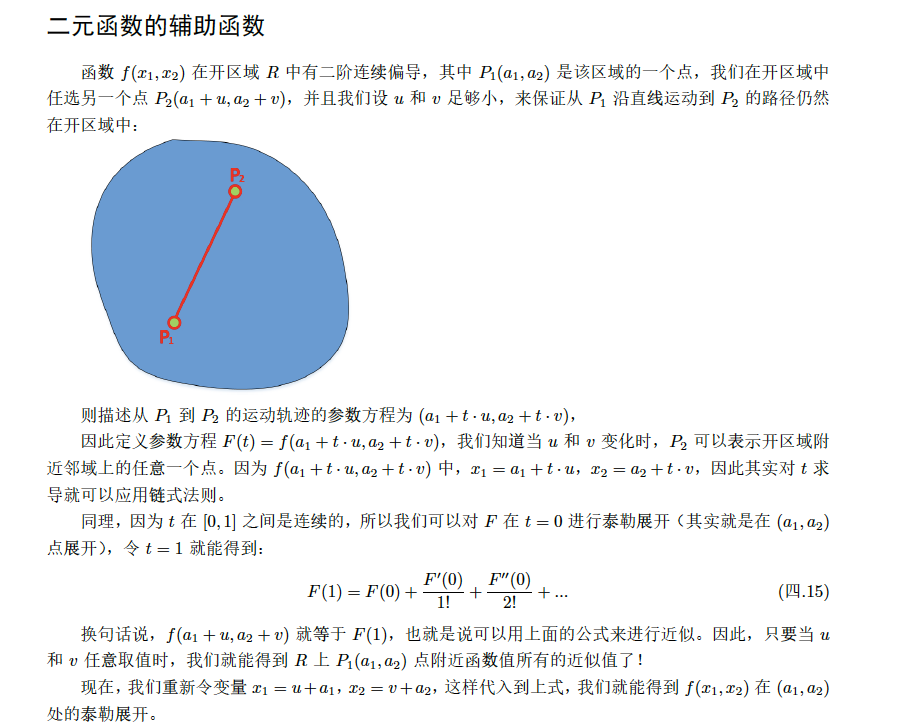
\includegraphics[scale=0.5]{figures/二元函数的辅助函数.png}
    \caption{二元函数的辅助函数}
\end{figure}

\section{小结}


函数在一点$a$展开,关注的是以$a$点附近邻域的函数的行为,肯定要满足在一点处的展开的值等于$a$处的函数值,所以泰勒级数中常数项等于$f(a)$,后面$n$阶导项等于$(x-a)^n$次方,当$x=a$时满足$f(x)=f(a)$。然后一阶导数项刚好用一条直线逼近。